\chapter{Implementation}
  \section{Data collection}
    This section contains details of the components built to access the accelerometer data and transfer it to a computer.
    
    Because both the smartwatch and the smartphone both run Android, it is possible to create components that are shared between the devices, reducing the amount of code I am required to write and to test, resulting in less redundancy, less complexity and ultimately a more reliable implementation. Both the \texttt{AccelerometerListenerService} and the \texttt{AccelerometerDataBlob} are shared between both devices.
    
    \subsection{Accessing the accelerometer}
      The \texttt{AccelerometerListenerService} is responsible for receiving readings from the accelerometer and delivering them to the data structure responsible for storage.
      
      As described in Section~\ref{sec:sensor-api}, the Sensor API utilises a listener methodology. It is required to create and register a listener that implements \texttt{onSensorChanged()}. 
      
      \subsubsection{Performance considerations}
        Because the accelerometer can update its values at a rate of over 50\si{Hz}, it is vital that any implementation of \texttt{onSensorChanged()} be non-blocking and ideally be very quick to execute. Any expensive computation or IO operation has to be moved to a separate thread.
        
        If the execution of \texttt{onSensorChanged()} takes longer than $\frac{1}{\mathrm{sample-rate}}$, requests for \texttt{onSensorChanged()} will queue and eventually lead to exhaustion of memory or dropping of data.
        
        For this reason the data structure used, discussed in Section~\ref{sec:storing-accelerometer-data}, is very lightweight and \texttt{onSensorChanged()} is only responsible for passing data to it.
      
      \subsubsection{Concurrency considerations}
        Because \texttt{onSensorChanged()} can be called at such a high rate, it is possible that new calls to the method can be made while previous calls are still executing. Data corruption could result from improper handling of asynchronicity.
      
        The documentation for the Sensor API is not explicit about whether calls to \texttt{onSensorChanged()} queue on the same thread or whether they can be dispatched asynchronously. For this reason, the \texttt{AccelerometerListenerService} was designed to be thread-safe by using Java concurrency primatives.
      
      \subsubsection{Power consumption considerations}
        Recording data from the accelerometer can be computationally expensive. This increase in computational overhead translates to an increase in power consumption in battery powered devices such as the smartphone and the smartwatch. It is for this reason that care should be taken to minimise power usage where possible while still collecting all the required data.
        
        One tradeoff that had to be made was between collection strategies. One strategy is to record data at a specified sample rate from when the recording is turned on until it is turned off. An alternative strategy is to record a window of data at set intervals and sleep the remainder of the time. For example, one might set the accelerometer to record 10 seconds of data every 50 seconds.
        
        Though this strategy saves battery power as the device turns off the accelerometer between recordings, a continous recording approach was taken in this project in order to have as much data as possible with which to train. In addition, the battery life was not severly impeded by the continous recording approach.
        
        Typically, Android will power off the display and later the CPU after a period of user-inactivity. Powering off the CPU means that the device will stop recording accelerometer data, and so it is required to maintain a wake-lock which keeps the CPU from powering off. It is also important to remember to release the wake-lock once accelerometer recording is complete. Otherwise, the device's CPU will remain on even when the device appears to be on standby, using battery.
        
      \subsubsection{Sampling rate}
        In ideal conditions, it would be sensible to sample at as fast a rate as possible: the resultant data can always be downsampled afterwards if it is not required. As per the Nyquist-Shannon sampling theory, discussed in Section~\ref{sec:intro-sig-processing}, our sample rate should be greater than twice the highest frequency of the signal. Because it isn't possible to know what the highest frequency is going to be, it would be reasonable to sample at a far higher rate. 
        
        However, picking a very fast sample rate in this context has two potential downsides: battery life drain and the size of resultant data. I investigated whether either battery life or the size of the resulting data would be a limiting factor of sample rate.
        
        The impact on power consumption of increasing the sample rate was negliable. One possible reason for this is that sampling using the accelerometer at all has high fixed costs and increasing the sample rate has lower marginal costs.
      
        Recall from Table~\ref{tab:data-row} that each measurement has a total size of 20 bytes. At a sample rate of 50\si{Hz}, we produce data at approximately 1 KBps or 3.6 MB per hour. The most memory-constrained device is the smartwatch, which only has 512 MB of RAM but 4 GB of internal storage. A data structure that stores the accelerometer data to the internal storage rather than to memory is required, but a sample rate of 50\si{Hz} produces a storable amount of data on reasonable-length activity recording.
        
        Another potential concern regarding data size is the transfer from the smartwatch to the smartphone. The only connection available is Bluetooth. The Bluetooth connection empircally has a maximum transfer rate of no more than 150 KBps, meaning an hour of activity data will take approximately 30 seconds to transfer.

    \subsection{Storing accelerometer data}
      \label{sec:storing-accelerometer-data}
      The data structure to hold the accelerometer data is required to be:
      \begin{itemize}
        \item \textbf{fast} because it will be accessed many times per second and cannot block;
        \item \textbf{on-disk} rather than in-memory, because the smartwatch may not have enough free memory to store all the accelerometer data for lengthy recordings;
        \item \textbf{thread-safe} as it is unclear whether calls to \texttt{onSensorChanged()} are queued or concurrent.
      \end{itemize}
      
      The data structure decided on was a temporary random-access file with buffered writing. The data is written as bytes through an output buffer. The output buffer is maintained in memory and is flushed when it reaches capacity. The capacity of the output buffer was set to 20000 bytes as data is only written in multiples of 20 bytes and the smartwatch is comfortably able to keep 20 kb in memory. This equates to data being saved to disk approximately every 20 seconds.
      
      % data structure – binary data
      % local temporary internal storage as opposed to memory
      % delete when transmitted
    \subsection{Transmitting accelerometer data}
      The accelerometer data has to be transmitted from the smartwatch to the smartphone before it can be transferred to a computer. As discussed in Section~\ref{sec:prep-data-api}, there are two methods to transfer data between the smartwatch and the smartphone: a DataItem and an Asset. Their advantages and disadvantages with respect to this project are highlighted in Table~\ref{tab:dataitem-vs-asset}.
      
      \begin{table}
        \centering
        {\tabulinesep=1.2mm
        \begin{tabu} to \linewidth { X[2,c,m] | X[3,l,m] | X[3,l,m] | }
          & \textbf{DataItem} & \textbf{Asset} \\
          \hline
          \textbf{Advantages} & 
            \begin{itemize}
              \item no separate data fetching step
              \item simpler, more reliable receiver code
              \item negligable transmission time
            \end{itemize} &
            \begin{itemize}
              \item no hard size limit
              \item can create an Asset from a File without storing it in memory
            \end{itemize} \\
          \hline
          \textbf{Disadvantages} &
            \begin{itemize}
              \item 100 KB size limit
              \item have to insert byte arrays
            \end{itemize} &
            \begin{itemize}
              \item some constructors don't seem to work
              \item transmission of large files takes a noticable amount of time
            \end{itemize} \\
          \hline
        \end{tabu}}
        \caption{Advantages and disadvantages of using the \texttt{DataItem} and \texttt{Asset} to transmit data from the smartwatch to the smartphone.}
        \label{tab:dataitem-vs-asset}
      \end{table}
      
      Because the DataItem has a 100 KB limit, an alternate transmission and storage system would have to have been built, where the smartwatch collects 100 KB of data and sends that to the smartphone while it continues to record. It is then reassembled at the smartphone receiver.
      
      I consider this solution inferior to the Asset implementation, which allows transmission of any size of data.
      % DataItem has 100kb limit.
      % Bug with Asset class – FileDescriptor
      % Use of Asset transmit
      % Sender
      % Receiver
    \subsection{User interface}
      \subsubsection{Smartphone}
      
      \subsubsection{Smartwatch}
      
  \section{Activities and data collection method}
    \subsection{Computer use}
    \subsection{Walking}
    \subsection{Cycling}
    \subsection{Standing}
    \subsection{Playing fussball}
    \subsection{Stair climbing}
  \section{Data processing}
    The data processing pipeline was written in Python, because of the strength of its numerical, statistical and machine learning libraries. The data processing was done on a computer as opposed to directly on the phone because of the computational demand required of training a classifier. In a real-world use-case, one could imagine classification occuring on a cloud server.
    \subsection{Importing and preprocessing}
      \subsubsection{Import}
        Each recording is stored in a separate binary file. The filename is always of the form: \texttt{<timestamp>-<recorder>-<device>-<activity.dat}. 
        
        NumPy includes methods to specify the types of binary data in a file and create an array from it. These are used to great effect to convert the binary data back into longs and floats.
        
        Access to the data files is then via a SQLite database, using the timestamp as the unique ID. The database allows easier access to individual records and, for example, all recordings of a certain activity.
        %read bytes
        %database
      \subsubsection{Preprocessing}
        Data is preprocessed before feature extraction.
        
        The first step is the drop the first and last 10 seconds of each data recording. The justification for this is that these accelerometer recordings will not actually be representative of the activity we are attempting to classify. Rather, they will primarily be recording the starting and ending of an activity.
        
        For each data recording, the magnitude of the acceleration $\|\mathbf{x}\| = \sqrt{x^2+y^2+z^2}$ was calculated. Patterns in the magnitude were found to be more distinguishing than any of the features extracted from the three axes individually. The magnitude is orientation-invariant, which gives better results when considering that a wrist may move in the same way but may be oriented slightly differently. In this scenario, periodicity will still be observed in the magnitude but may not be observed in each of the three axes individually.
        
        Data is then filtered. As discussed in Section~\ref{sec:intro-sig-processing}, the data recorded by the accelerometer is subject to noise. Reducing the effect of this noise will produce a signal in which it is easier to observe the underlying patterns produced by movement.
        
        A fifth-order Butterworth Filter with a critical frequency of 5 \si{Hz} was used. The Butterworth Filter was chosen because it has no gain ripple in the pass band or the stop band and because the slow cutoff is not a problem for our application, as the frequencies of activities we are concerned with are far less than the frequency of the noise. A graph of the frequency responses for several Butterworth Filters is given in Figure~\ref{fig:butterworth_filters}.
        
        \begin{figure}
          \centering
          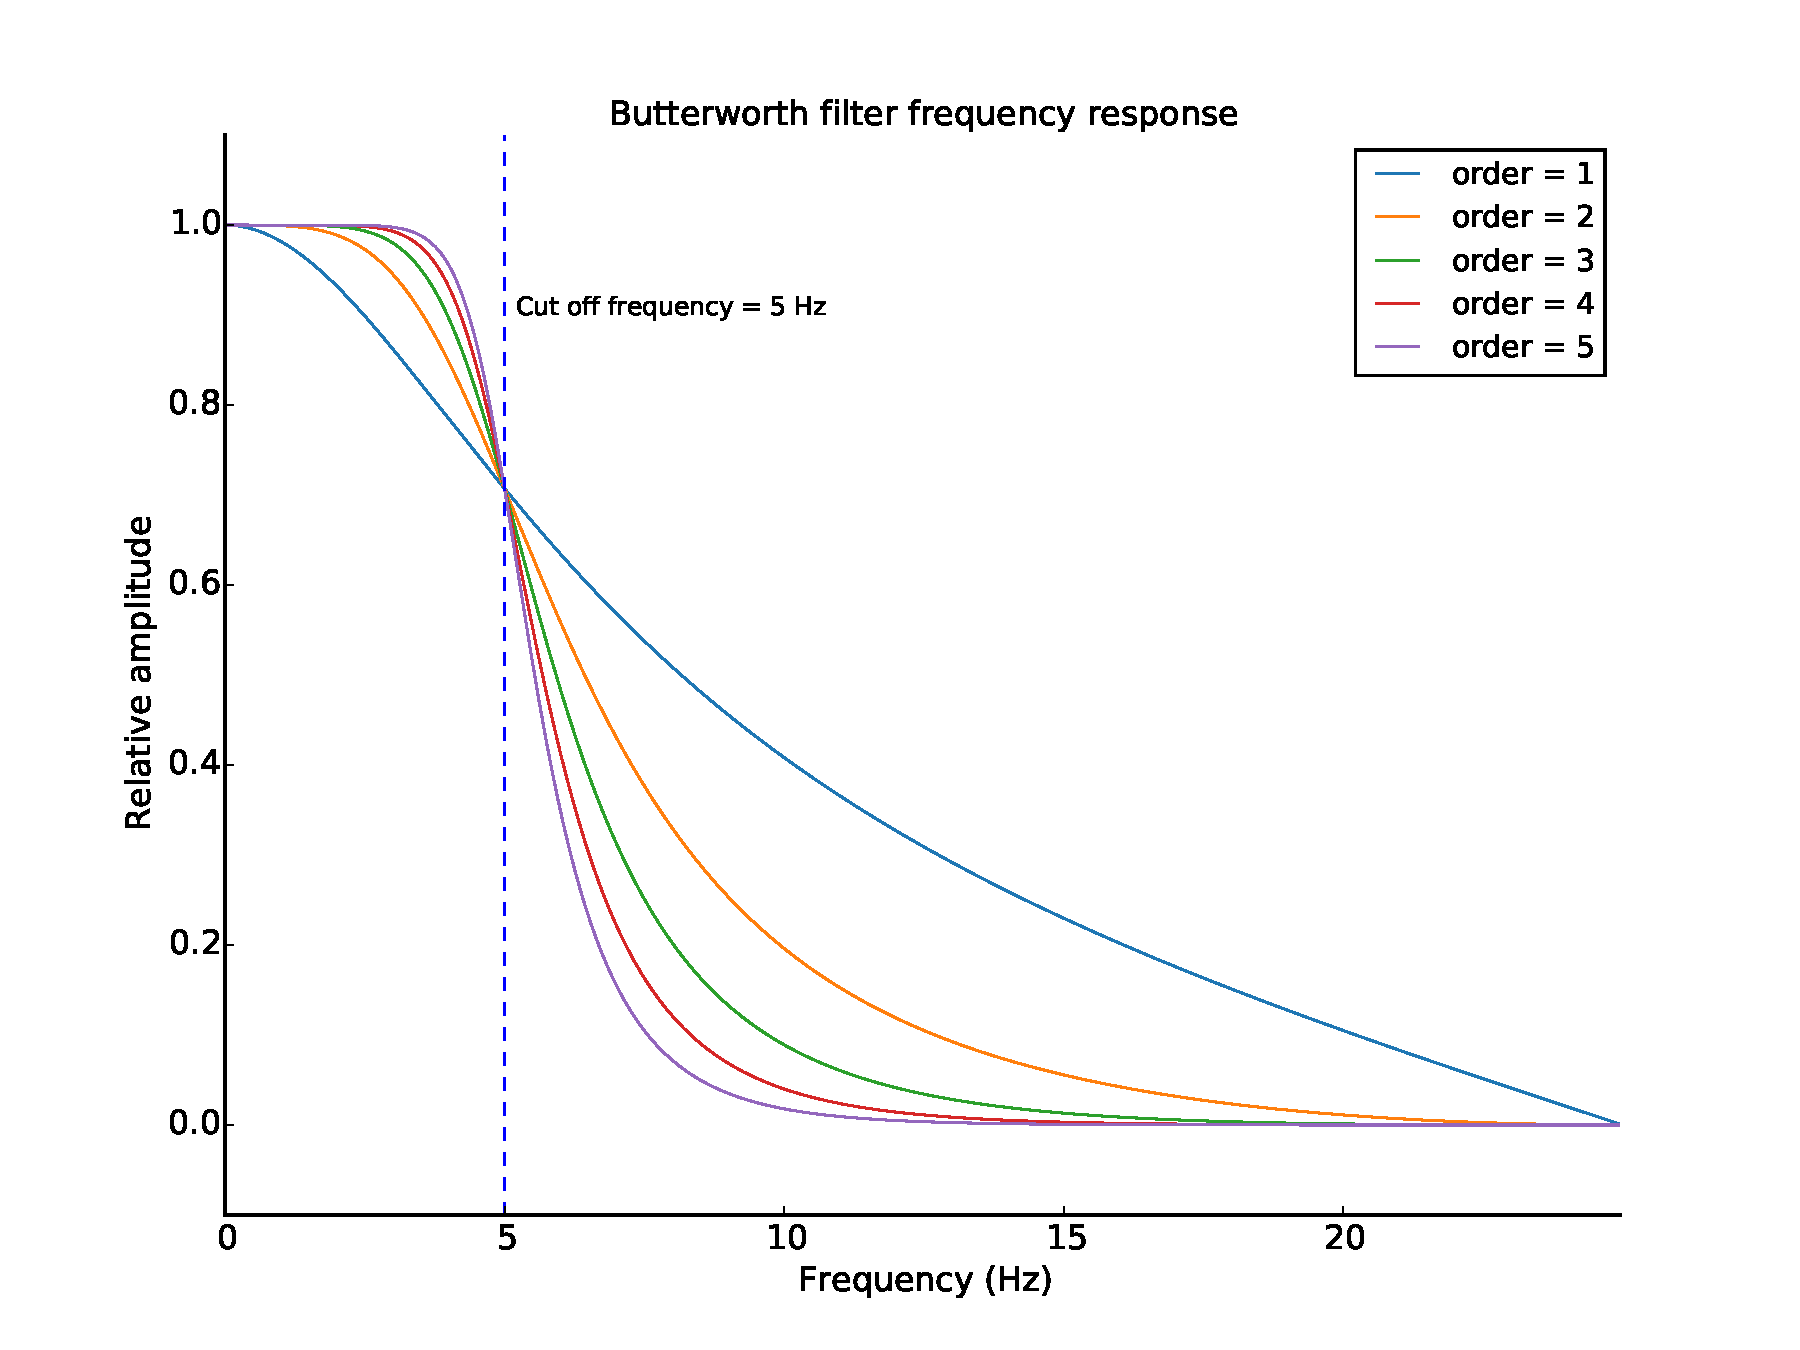
\includegraphics[width=1.0\textwidth]{butterworth_filters}
          \caption{Frequency response for Butterworth filters of different orders. Each has a critical frequency of 5 \si{Hz}. A fifth-order Butterworth filter was used to filter the noise from the accelerometer data.}
          \label{fig:butterworth_filters}
        \end{figure}
        
        %disregard first and last 10 seconds
        %magnitude
        %filtering
      \subsubsection{Windows}
        Each data recording is split into 10 second windows. Features are extracted from each of these bins individually. Splitting into windows allows the production of multiple feature rows from the same recording. In theory, every window for a particular activity should exhibit extracted features that are consistent. A 10 second window was picked as a balance between producing enough feature rows from collected data and ensuring that several cycles of an activity were included. 
      
        %10 second overlapping bins
    \subsection{Feature extraction}
      In total, 22 features are extracted from each window. The smartwatch and smartphone data are treated as separate windows for the purposes of feature extraction. A summary of the extracted features is given in Table~\ref{tab:extracted-features}. This section goes on to describe and justify each of these features.
      
      \begin{table}
        \centering
        {\tabulinesep=1.2mm
        \begin{tabu} to \linewidth { c X[c]}
          \textbf{No of features} & \textbf{Description of each feature} \\
          \hline
          4 & Mean of each axis and magnitude \\
          4 & Standard deviation of each axis and magnitude \\
          4 & Maximum amplitude of each axis and magnitude \\
          4 & Median absolute deviation of each axis and magnitude \\
          3 & Pairwise correlation coefficient of each of the three axes \\
          1 & Spectral flatness of magnitude \\
          1 & Spectral entropy of magnitude \\
          1 & Frequency of maximum amplitude in the power spectrum of the magnitude \\
          \hline
        \end{tabu}}
        \caption{A summary of extracted features.}
        \label{tab:extracted-features}
      \end{table}
      
      \subsubsection{Mean of each axis and magnitude}
        The arithmetic mean $\bar{X}$ defined as $$\bar{X} = \frac{1}{n}\sum\limits_{i = 1}^{n}x_i$$ was calculated for each of the x, y and z axes and also for the magnitude.
        
        The arithmetic mean does not encode a lot of data, but is useful for determining primary orientation during the activity. For example, computer use has a z mean which is close to gravitational accleration while the others are near zero. This indicates the devices primarily points upward during this activity.
      
      \subsubsection{Standard deviation of each axis and magnitude}
        The standard deviation $\sigma$ defined as $$\sigma = \sqrt{\frac{1}{n}\sum\limits_{i = 1}^{n}(\bar{x}-x_i)^2}$$ was calculated for each of the x, y and z axes and also for the magnitude.
        
      \subsubsection{Maximum amplitude of each axis and magnitude}
        The maximum $x_{\max}$ defined as $$x_{\max} = \max_i x_i $$
      \subsubsection{Mean average deviation of each axis and magnitude}
        The mean average deviation $x_\mathrm{mad}$ defined as $$x_\mathrm{mad} = \mathrm{median}_i (|x_i - \mathrm{median}_j(x_j)|)$$
      \subsubsection{Pairwise correlation coefficient of each of the three axes}
        The covariance is a measure of how much two random variables change together. The covariance of two random variables $X$ and $Y$, $\mathrm{Cov}(X, Y)$ is defined as $$\mathrm{Cov}(X, Y) = \mathbb{E}[(X - \bar{X})(Y - \bar{Y})]$$
        
        The correlation coefficient, $\mathrm{Cor(X,Y)}$, of two random variables $X$ and $Y$ is the normalised covariance of the two random variables. $$\mathrm{Cor(X,Y)} = \frac{\mathrm{Cov(X,Y)}}{\sigma_{\mathrm{X}}\sigma_{\mathrm{Y}}}$$
        
        $\mathrm{Cor(X,Y)}$ has a value between $-1$ and $1$, with $1$ representing total positive correlation, $0$ representing no correlation and $-1$ representing total negative correlation.
         
        The correlation coefficient was calculated for each pair of axes, producing three features: $\mathrm{Cor(X,Y)}$, $\mathrm{Cor(X,Z)}$, and $\mathrm{Cor(Y,Z)}$. The correlation coefficients give a measure of how much the axes move together during the recording. This encodes some information about the direction of movement.
      \subsubsection{Spectral flatness of magnitude}
        Spectral flatness is also known as the tonality coefficient. It is a measure of how noise-like or tone-like a signal is. White noise has a spectral flatness approaching 1, while a pure tone has a spectral flatness approaching zero.
        
        Spectral flatness is calculated from the power spectrum of the signal. Recall from Section~\ref{sec:intro-sig-processing} that the power spectrum is the squared magnitude of the Fourier transform of the signal.
        
        If $x_i$ represents the magnitude in the power spectrum of bin $i$, then the Flatness of a power spectrum $X = [x_1, x_2, \dots , x_N]$ is defined as
        
        $$\mathrm{Flatness(X)} = \frac{\sqrt[N]{\prod\limits_{i=1}^N x_i}}{\frac{1}{N}\sum_{i=1}^N x_i}$$
        
        The geometric mean can be expressed as a summation of logarithms rather than a product, giving an alternative formula for the Flatness that does not require a large product or an nth root. As our Fourier transforms are likely to be over 10000 elements long, avoiding the large product or the expensive nth root calculation is desirable. Following conversion to a logarithmic summation, the Flatness is:
        
        $$\mathrm{Flatness(X)} = \frac{\exp \left( \frac{1}{N}\sum\limits_{i=1}^N \ln x_i \right) }{\frac{1}{N}\sum_{i=1}^N x_i}$$
        
        Spectral flatness gives a measure of how periodic a signal is. Activities where there is very high spectral flatness, akin to white noise, are aperiodic. For example, fussball and standing have no associated period, while walking when measured through the smartphone has a clear period.
      \subsubsection{Spectral entropy of the magnitude}
        The spectral entropy of a signal is calculated as the entropy of its power spectrum. It is defined as:

        $$\mathrm{entropy} = -\sum\limits_{i=1}^N x_i \log_2 x_i$$
      \subsubsection{Frequency of maximum amplitude in the power spectrum of the magnitude}
        The power spectrum of the magnitude shows at which frequencies the power in the signal is distributed. It is defined as the squared magnitude of the Fourier transform of the signal.
        
        Rather than take the Fourier transform of the orginal signal, the mean of the signal was first subtracted. If the original signal oscillates about some non-zero offset, the Fourier transform will have a spike at the origin (0 \si{Hz}, or the DC component). To avoid incorrectly classing 0 \si{Hz} as the maximum, we subtract the mean from the original signal. The frequency of maximum amplitude of a power spectrum $X$ is then:
        
        $$\mathrm{f}_\mathrm{max} = \operatorname*{arg\,max}_f X_f$$
        
    \subsection{Machine learning}
  \section{Summary}
